\documentclass[tikz,border=0pt,11pt]{standalone}
\usepackage[T1]{fontenc}
\usepackage[utf8]{inputenc}
\usepackage{lmodern,amsmath,amssymb}
\usepackage[swedish]{babel}
\usetikzlibrary{arrows.meta,calc,positioning,decorations.pathmorphing,decorations.pathreplacing,patterns,shadings}
\definecolor{navy}{HTML}{102F40}
\definecolor{teal}{HTML}{147D78}
\definecolor{lightteal}{HTML}{E6F1ED}
\definecolor{gold}{HTML}{B88B3B}
\definecolor{palegold}{HTML}{F7EEDB}
\definecolor{rust}{HTML}{B6533B}
\definecolor{palerust}{HTML}{FAEAE4}
\definecolor{paper}{HTML}{F7F5EE}
\definecolor{muted}{HTML}{5B6D72}
\definecolor{line}{HTML}{D6DED8}
\renewcommand{\familydefault}{\sfdefault}
\newcommand{\atom}[5]{\shade[ball color=#3!70] (#1,#2) circle (#5);\node[text=white,font=\bfseries\small] at (#1,#2){#4};}
\newcommand{\water}[3]{\begin{scope}[shift={(#1,#2)},scale=#3]\draw[navy!45,line width=2pt] (-.3,.22)--(0,0)--(.3,.22);\atom{0}{0}{rust}{O}{.22}\atom{-.3}{.22}{teal}{H}{.15}\atom{.3}{.22}{teal}{H}{.15}\end{scope}}
\newcommand{\panel}[4]{\filldraw[fill=white,draw=line,rounded corners=5pt] (#1,#2) rectangle ++(#3,#4);}
\newcommand{\note}[4]{\node[txt,text width=#3cm] at (#1,#2){#4};}
\tikzset{txt/.style={anchor=north west,align=left,text=navy,font=\small},
 head/.style={anchor=west,text=navy,font=\bfseries\large},
 label/.style={align=center,text=navy,font=\small},
 smalllabel/.style={align=center,text=muted,font=\footnotesize},
 arrow/.style={-{Latex[length=2.5mm,width=1.8mm]},line width=1.2pt,draw=teal},
 goldarrow/.style={-{Latex[length=2.5mm]},line width=1.2pt,draw=gold},
 rustarrow/.style={-{Latex[length=2.5mm]},line width=1.2pt,draw=rust},
 dashedarrow/.style={arrow,dashed},
 badge/.style={fill=lightteal,rounded corners=3pt,text=teal,font=\bfseries\small,inner sep=5pt}}
\begin{document}
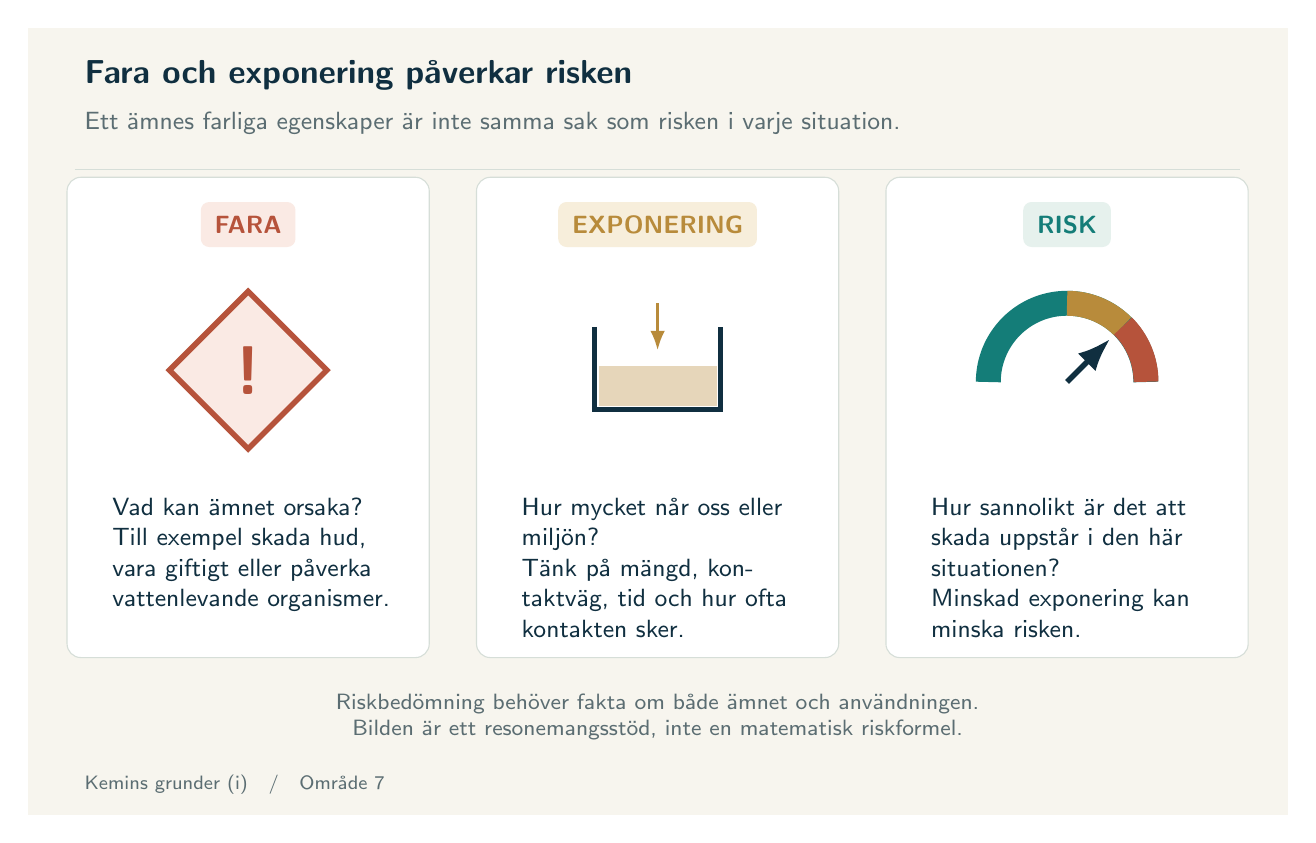
\begin{tikzpicture}[x=1cm,y=1cm]
\path[use as bounding box] (0,0) rectangle (16,10);
\fill[paper] (0,0) rectangle (16,10);
\node[head] at (.6,9.4){Fara och exponering påverkar risken};
\note{.6}{9.05}{14.8}{\textcolor{muted}{Ett ämnes farliga egenskaper är inte samma sak som risken i varje situation.}}
\draw[line] (.6,8.2)--(15.4,8.2);

\panel{.5}{2}{4.6}{6.1}\panel{5.7}{2}{4.6}{6.1}\panel{10.9}{2}{4.6}{6.1}
\node[badge,fill=palerust,text=rust] at (2.8,7.5){FARA};\node[badge,fill=palegold,text=gold] at (8,7.5){EXPONERING};\node[badge] at (13.2,7.5){RISK};
\draw[rust,fill=palerust,line width=2pt] (2.8,6.65)--(3.8,5.65)--(2.8,4.65)--(1.8,5.65)--cycle;\node[text=rust,font=\bfseries\Huge] at (2.8,5.65){!};
\draw[navy,line width=2pt] (7.2,6.2)--(7.2,5.15)--(8.8,5.15)--(8.8,6.2);\fill[gold!35] (7.25,5.2) rectangle(8.75,5.7);\draw[goldarrow] (8,6.5)--(8,5.9);
\draw[teal,line width=9pt] (12.2,5.5) arc(180:0:1);\draw[gold,line width=9pt] (13.2,6.5) arc(90:45:1);\draw[rust,line width=9pt] (13.91,6.21) arc(45:0:1);\draw[navy,line width=2pt,-{Latex}] (13.2,5.5)--(13.75,6.05);
\note{.95}{4.15}{3.75}{Vad kan ämnet orsaka?\par Till exempel skada hud, vara giftigt eller påverka vattenlevande organismer.}
\note{6.15}{4.15}{3.75}{Hur mycket når oss eller miljön?\par Tänk på mängd, kontaktväg, tid och hur ofta kontakten sker.}
\note{11.35}{4.15}{3.75}{Hur sannolikt är det att skada uppstår i den här situationen?\par Minskad exponering kan minska risken.}
\node[smalllabel,text width=14cm] at (8,1.25){Riskbedömning behöver fakta om både ämnet och användningen. Bilden är ett resonemangsstöd, inte en matematisk riskformel.};\node[anchor=west,text=muted,font=\scriptsize] at (.6,.38){Kemins grunder (i)\quad /\quad Område 7};

\end{tikzpicture}\end{document}
